\chapter{Experiment}
\label{sec:experiment}
This section is devoted to demonstrate the superiority of the proposed method in terms of whether the proposed method can further incorporate the characteristics of reflectance and illumination with the cost function of the minimization optimization problem, and whether it can naturally enhance low-light images. The word "naturally" means that the methods can suppress over-enhancement and noise amplification when enhancing. To this aim, this section is composed of the subsequent six aspects: testing datasets, competing methods, decomposition comparison, qualitative evaluation, quantitative evaluation, and parameter study.
In this experiment, the empirical parameters are set $\alpha=0.01$, $\beta=0.01$, $\gamma=0.25$, $\epsilon=10^{-2}$. In addition, the proposed method is performed on Python implementation on PC with 16GB RAM, Intel Core i7-6700 CPU @ 3.40GHz. 

\section{Testing Datasets} \label{sec:dataset}
Since we can not obtain the ground truth for low light images in actual applications, we selected $21$ image datasets among many datasets which various researches \cite{wvm}, \cite{lime}, \cite{jiep} on low-light image enhancement have employed. Fig.\ref{fig:dataset} shows the datasets used in the following experiment. The images contain different scenes, such as statue, buildings, Street lamps, landscape, people, sunset, and etc.
\begin{figure}[tb]
	\centering
	\includegraphics[width=1.0\hsize]{images/experiment/dataset1.eps}
	\caption{$21$ image datasets which are captured at diversified locations.} \label{fig:dataset}
\end{figure}

\section{Competing Methods} \label{sec:competition}
In this research, five state-of-the-art methods are collected, which can be divided into two types. The first type is composed of Retinex-based model, namely simultaneous reflectance and illumination estimation (SRIE) \cite{srie}, a weighted variational model (WVM) \cite{wvm}, a robust Retinex model (RRM) \cite{rrm}, and a joint intrinsic-extrinsic prior (JieP) \cite{jiep}. These methods are based on variational Retinex model, and can simultaneously estimate reflectance and illumination. In addition, SRIE, WVM, and JieP are performed on HSV-color space as well as the proposed method. The second type is composed of non-Retinex model, namely low-light image enhancement via illumination map estimation (LIME) \cite{lime}. This method is based on dehazing model and enhances low-light images by estimating the transmission map using the energy function. Programming codes of all methods are downloaded from the author's websites such as Github and implemented with the recommended experimental settings.

\section{Decomposition Comparison} \label{sec:decomposition}
The aim of this section is to evaluate how accurately the proposed method estimates reflectance and illumination. It is assumed in \cite{retinex} that illumination should not distort the structure information while keeping smoothness, and reflectance should contain rich detail of an observed image. Negative effects such as halo artifacts, noise amplification, and over-enhancement generate when the methods cannot sufficiently consider the assumption. Therefore, it is necessary to evaluate how much further the methods can consider the characteristics of refllectance and illumination. However, we can not obtain the ground truth for reflectance and illumination in actual applications. Thus, in order to confirm the effectiveness of the proposed method, the proposed method is compared with SRIE, WVM, and JieP because these methods are based on Retinex model and are implemented on HSV-color space as well as the proposed method.\par
Fig.\ref{fig:decomposition} summarizes the decomposition results of reflectance and illumination in different methods. SRIE cannot significantly distinguish between reflectance and illumination component, so that the estimated reflectance contains little textures detail. WVM sufficiently reveals textures detail in the estimated reflectance, but amplifies noise in dark regions. Moreover, the methods over-smooth illumination, so that the estimated reflectance generates halo artifacts in edges of buildings. JieP sufficiently removes illumination component from reflectance, but the estimated illumination loses the meaningful structure information too much. As a result, the estimated reflectance generates halo artifacts in edges of buildings. Moreover, the estimated reflectance contains much noise in dark regions. In summary, the proposed method can sufficiently maintain the structure information with less textures detail in the estimated illumination. In addition, the proposed method can reveal fine textures detail while suppressing halo artifacts, noise amplification, and over-enhancement in the estimated reflectance.
%----反射と照明の推定比較---- %
\begin{figure}[htbp]
\centering
	\begin{minipage}[b]{0.49\hsize}
		\centering
		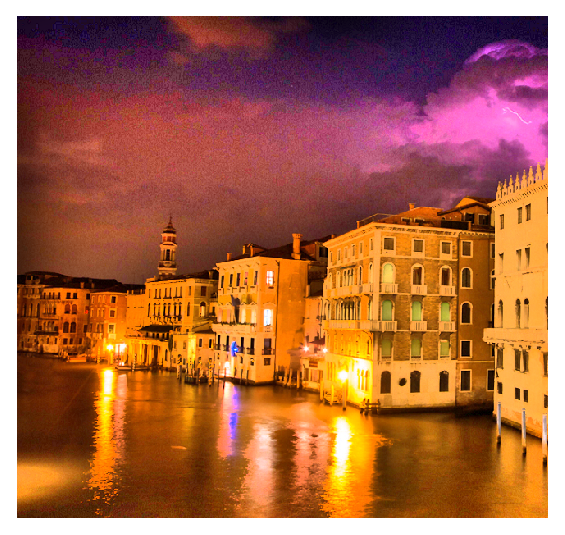
\includegraphics[width=55mm, height=45mm]{images/experiment/decomp1/srie/reflectance.eps}
	\end{minipage}
	\begin{minipage}[b]{0.49\hsize}
		\centering
		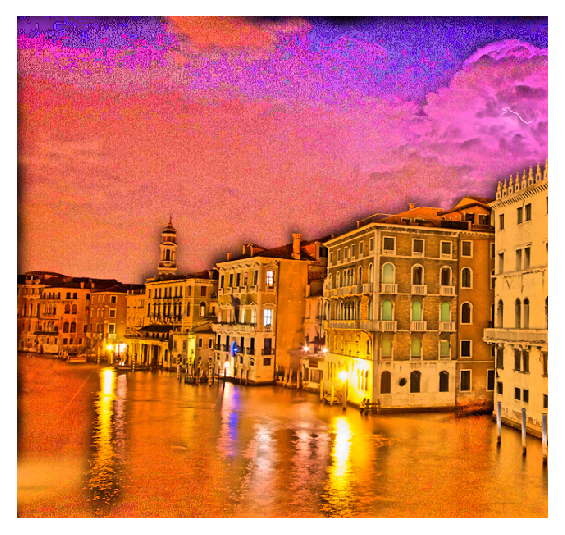
\includegraphics[width=55mm, height=45mm]{images/experiment/decomp1/wvm/reflectance.eps}
	\end{minipage}\\
	\vspace{1.5mm}
	\begin{minipage}[b]{0.49\hsize}
		\centering
		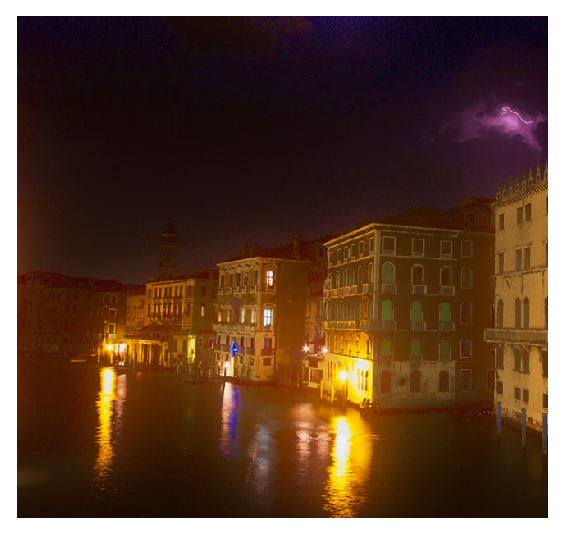
\includegraphics[width=55mm, height=45mm]{images/experiment/decomp1/srie/illumination.eps}
		\subcaption{SRIE} \label{fig:decomp_srie}
	\end{minipage}
	\begin{minipage}[b]{0.49\hsize}
		\centering
		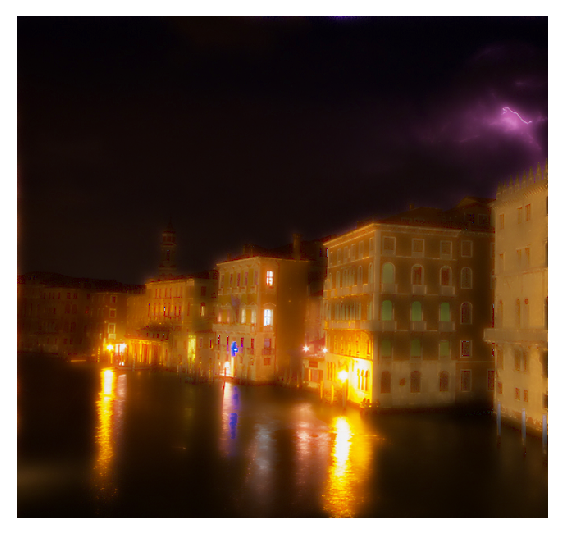
\includegraphics[width=55mm, height=45mm]{images/experiment/decomp1/wvm/illumination.eps}
		\subcaption{WVM} \label{fig:decomp_wvm}
	\end{minipage}
	\begin{minipage}[b]{0.49\hsize}
		\centering
		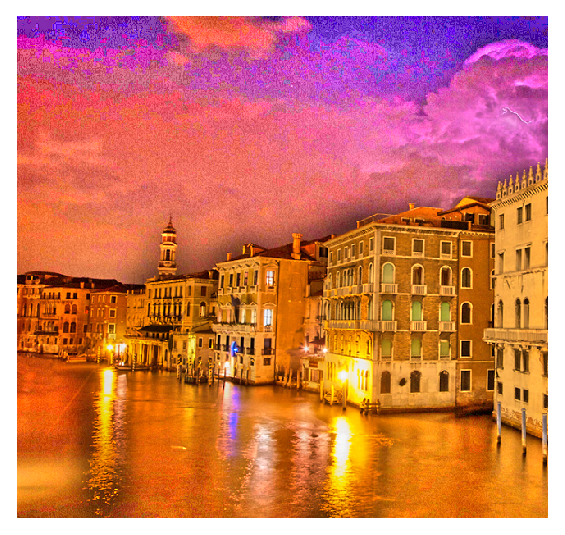
\includegraphics[width=55mm, height=45mm]{images/experiment/decomp1/jiep/reflectance.eps}
	\end{minipage}
	\begin{minipage}[b]{0.49\hsize}
		\centering
		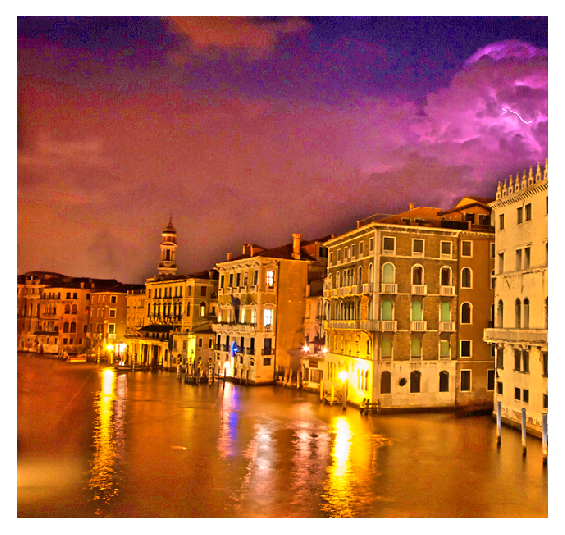
\includegraphics[width=55mm, height=45mm]{images/experiment/decomp1/prop/reflectance.eps}
	\end{minipage}\\
	\vspace{1.5mm}
	\begin{minipage}[b]{0.49\hsize}
		\centering
		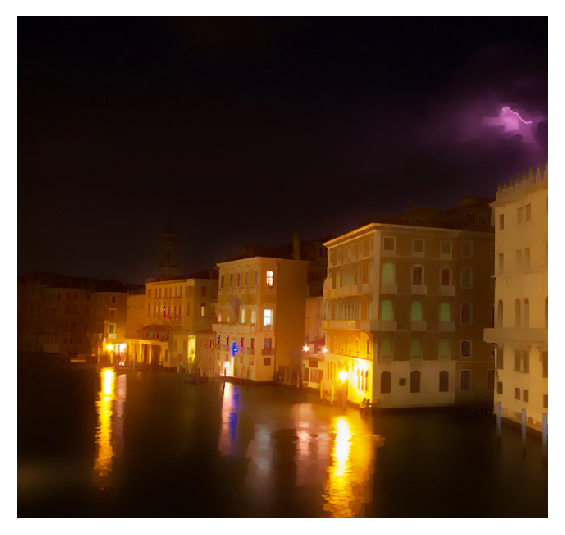
\includegraphics[width=55mm, height=45mm]{images/experiment/decomp1/jiep/illumination.eps}
		\subcaption{JieP} \label{fig:decomp_jiep}
	\end{minipage}
	\begin{minipage}[b]{0.49\hsize}
		\centering
		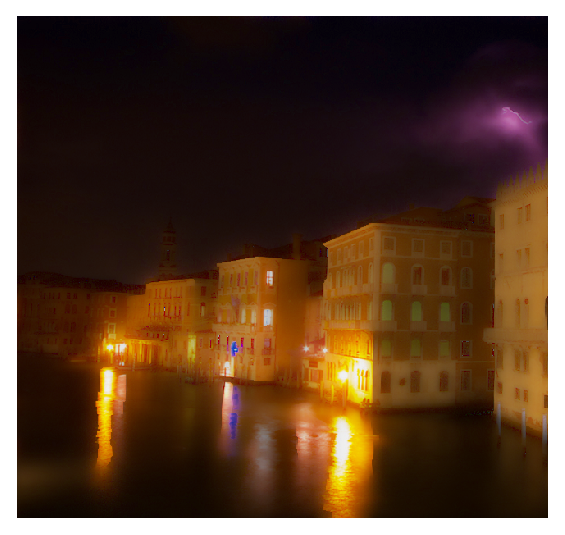
\includegraphics[width=55mm, height=45mm]{images/experiment/decomp1/prop/illumination.eps}
		\subcaption{Ours} \label{fig:decomp_prop}
	\end{minipage}
	\caption{Reflectance and illumination for different methods.((a)-(d) top: reflectance, bottom: illumination)}
	\label{fig:decomposition}
\end{figure}

\section{Qualitative Evaluation} \label{sec:qualitative}
This section focuses on the comparison based on the qualitative evaluation. 
In the qualitative evaluation, the discussion centers on whether the methods can enhance low-light images naturally and significantly. Similar to the above comparison of decomposition, several state-of-the-art methods are used: three Retinex methods including SRIE, WVM, and RRM; non-Retinex method (LIME). \par
Fig.\ref{fig:qualitative/1} summarizes the enhancement results of all the methods for dataset $\#6$.
The dataset $\#6$ has two features. One is  that the enhanced image usually generates halo artifacts in edges of buildings. The other is that the enhanced image tends to lose textures detail in the right tower which contains high intensities in the entire image. SRIE and WVM generate noticeable halo artifacts in the edges of the tower. In addition, these methods lose textures detail because these methods cannot significantly decompose the low-light image into reflectance and illumination and prevent the awareness of textures detail. 
RRM exhibits an outstanding performance in suppression of halo effects and contrast enhancement, but the result of this method is likely to be blurry and loses textures detail.
LIME shows impressive performance in lighting up dark regions. However, the method often over-enhances the low-light image, so that the enhanced image loses textures detail too much, specifically in bright regions. 
In summary, the proposed method can suppress halo artifacts and over-enhancement. Moreover, the proposed method clarifies more textures detail even in bright regions.\par
Fig. \ref{fig:qualitative/2} summarizes the enhancement results of all the methods for dataset $\#7$. The dataset $\#7$ has two features. One is that the over-enhances is usually caused in bright regions. The other is that noise tends to be amplified in dark regions. SRIE can naturally enhance the low-light image, but this method can not sufficiently help the awareness of textures detail. WVM satisfactorily enhances the low-light image, but generates severe noise amplification in dark regions. RRM performs image enhancement while suppressing noise amplification, but the generated image is too smooth and is over-enhanced on the entire image. LIME illuminates dark regions, but over-enhances bright regions.
In summary, the proposed method achieves good performances in image enhancement, the awareness of textures detail, and suppression of noise amplification and over-enhancement.
%----定性評価1の図---- %
\begin{figure}[htbp]
\centering
	\begin{minipage}[b]{0.49\hsize}
		\centering
		\includegraphics[width=66mm, height=42mm]{images/experiment/qualitative/comp1/1/input.eps}
		\subcaption{Low-light Image} \label{fig:qualitative/1/input}
	\end{minipage}
	\begin{minipage}[b]{0.49\hsize}
		\centering
		\includegraphics[width=66mm, height=42mm]{images/experiment/qualitative/comp1/1/srie.eps}
		\subcaption{SRIE} \label{fig:qualitative/1/srie}
	\end{minipage} 
	\begin{minipage}[b]{0.49\hsize}
		\centering
		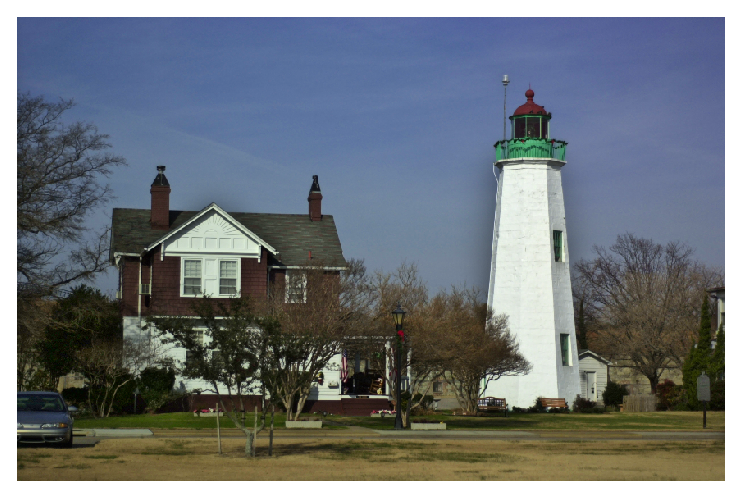
\includegraphics[width=66mm, height=42mm]{images/experiment/qualitative/comp1/1/wvm.eps}
		\subcaption{WVM} \label{fig:qualitative/1/wvm}
	\end{minipage}
	\begin{minipage}[b]{0.49\hsize}
		\centering
		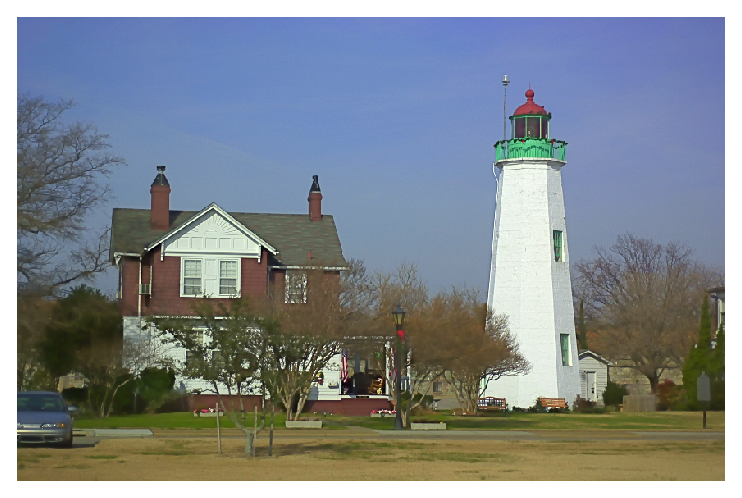
\includegraphics[width=66mm, height=42mm]{images/experiment/qualitative/comp1/1/rrm.eps}
		\subcaption{RRM} \label{fig:qualitative/1/rrm}
	\end{minipage} 
	\begin{minipage}[b]{0.49\hsize}
	\centering
	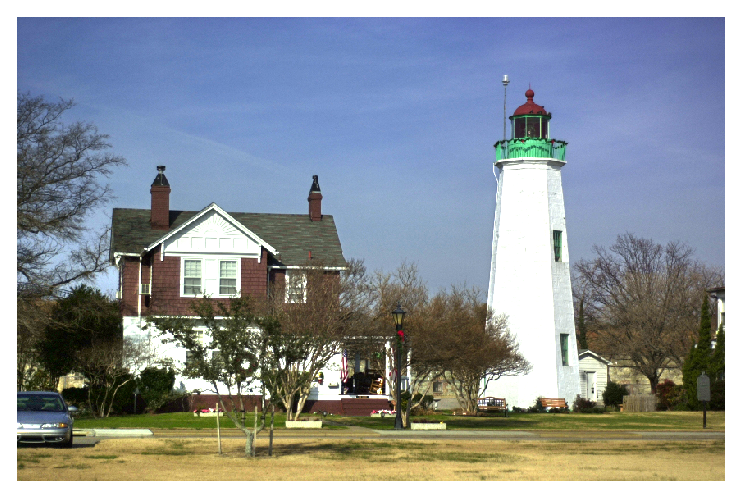
\includegraphics[width=66mm, height=42mm]{images/experiment/qualitative/comp1/1/lime.eps}
	\subcaption{LIME} \label{fig:qualitative/1/lime}
	\end{minipage}
	\begin{minipage}[b]{0.49\hsize}
	\centering
	\includegraphics[width=66mm, height=42mm]{images/experiment/qualitative/comp1/1/prop.eps}
	\subcaption{Ours} \label{fig:qualitative/1/prop}
	\end{minipage}
	\caption{Comparison of low-light image enhancement results for test image $\#6$.}
	\label{fig:qualitative/1}
\end{figure}
%----定性評価2の図---- %
\begin{figure}[htbp]
\centering
	\begin{minipage}[b]{0.49\hsize}
		\centering
		\includegraphics[width=64mm, height=48mm]{images/experiment/qualitative/comp2/2/input.eps}
		\subcaption{Low-lgiht Image} \label{fig:qualitative/2/input}
	\end{minipage}
	\begin{minipage}[b]{0.49\hsize}
		\centering
		\includegraphics[width=64mm, height=48mm]{images/experiment/qualitative/comp2/2/srie.eps}
		\subcaption{SRIE} \label{fig:qualitative/2/srie}
	\end{minipage} \\
	\begin{minipage}[b]{0.49\hsize}
		\centering
		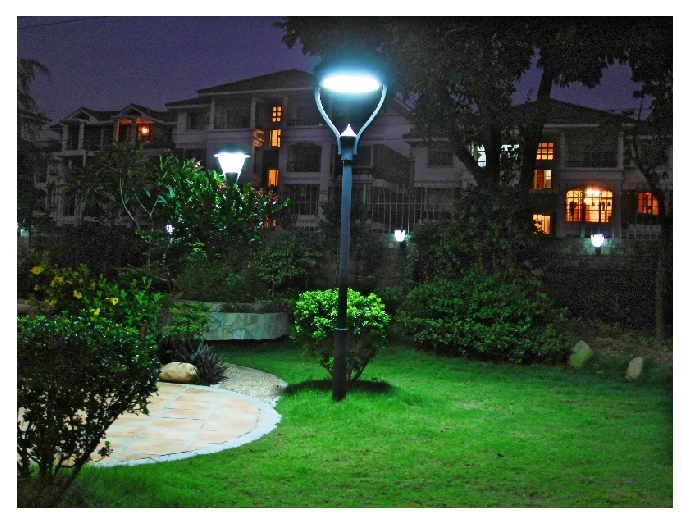
\includegraphics[width=64mm, height=48mm]{images/experiment/qualitative/comp2/2/wvm.eps}
		\subcaption{WVM} \label{fig:qualitative/2/wvm}
	\end{minipage}
	\begin{minipage}[b]{0.49\hsize}
		\centering
		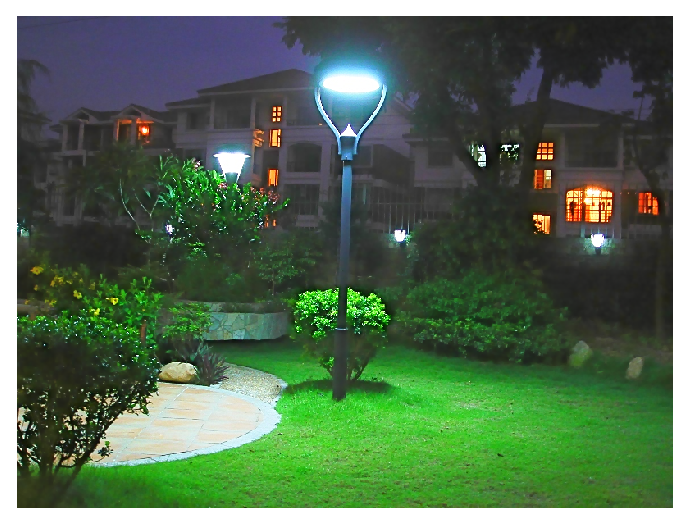
\includegraphics[width=64mm, height=48mm]{images/experiment/qualitative/comp2/2/rrm.eps}
		\subcaption{RRM} \label{fig:qualitative/2/rrm}
	\end{minipage} \\
	\begin{minipage}[b]{0.49\hsize}
	\centering
	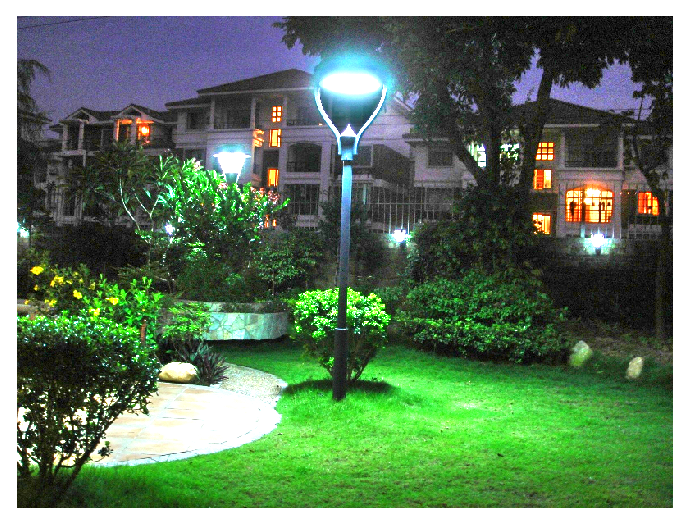
\includegraphics[width=64mm, height=48mm]{images/experiment/qualitative/comp2/2/lime.eps}
	\subcaption{LIME} \label{fig:qualitative/2/lime}
	\end{minipage}
	\begin{minipage}[b]{0.49\hsize}
	\centering
	\includegraphics[width=64mm, height=48mm]{images/experiment/qualitative/comp2/2/prop.eps}
	\subcaption{Ours} \label{fig:qualitative/2/prop}
	\end{minipage}
	\caption{Comparison of low-light image enhancement results for test image $\#7$.}
	\label{fig:qualitative/2}
\end{figure}

\section{Quantitative Evaluation} \label{sec:quantitative}
This section focuses on the comparison with the proposed method and several state-of-the-art methods in terms of two quantitative evaluations: lightness order error (LOE) \cite{loe} and autoregressive-based image sharpness metric (ARISM) \cite{arism}. The evaluations indicate naturalness of the enhanced image. The smaller the score of the evaluations are, the better an enhanced image preserves naturalness of lightness.\par
\subsection{Lightness Order Error}
As pointed out in \cite{loe}, the relative order of lightness represents the light source directions and the lightness variation, since the naturalness of an enhanced image is related to the relative order of lightness in different local areas. LOE measures the lightness distortion of enhanced images as follows:
\begin{equation}
\mbox{LOE} = \frac{1}{m} \sum_{x=1}^{m}{RD(x)}, \label{eq:loe}
\end{equation}
where $m$ is the pixel number. Here $RD(x)$ is the relative order difference of the lightness between an observed image $S$ and the enhanced image $S^{'}$ for pixel $x$, defined by
\begin{equation}
RD(x) = \sum_{y=1}^{m}F(B(x), B(y)) \oplus F(B^{'}(x), B^{'}(y)), \label{eq:rd}
\end{equation}
where $\oplus$ stands for the exclusive-or operator, $B(x)$ and $B^{'}(x)$ are the bright channel of an observed image and the enhanced image at the location $x$, respectively. The function $F(p, q)$ returns $1$ if $q \in p$, $0$ otherwise. As suggested in \cite{lime}, down-sampling is needed to reduce the complexity of computing LOE. Therefore, when evaluating LOE, all images are down-sampled to $50 \times 50$.\par
As shown in Fig. \ref{fig:loe} and Table \ref{tab:loe}, the proposed method outperforms the others in almost all images. This means that the proposed method can keep the naturalness of images well when enhancing. The proposed method sufficiently suppresses halo artifacts, noise amplification and over-enhancement, since the proposed method incorporates the characteristics of reflectance and illumination with the optimization equation. In other words, the mixture $L_{2}$ - $L_{P}$ variational Retinex model and the adaptive texture map contribute to alleviation on such negative effects. 
%----LOEの平均図---- %
\begin{figure}[tb]
	\centering
	\includegraphics[width=125mm, height=100mm]{images/experiment/quantitative/loe.eps}
	\caption{Comparison of the average score in the LOE for different methods.} \label{fig:loe}
\end{figure}
%----LOEのランキング表---- %
\begin{table}[htbp]
	\begin{center} 
	\caption{The number of images in each rank based on LOEs.}
	\begin{tabular}{c||c|c|c|c|c|c} \hline
	\backslashbox{\bf{Rank}}{\bf{Method}} & {SRIE} & {WVM} & {LIME} & {RRM} & {JieP} & {Ours} \\ \hline \hline
	\textbf{1st} & 6 & 0 & 2 & 1 & 0 & 12  \\ \hline
	\textbf{2nd} & 10 & 1 & 3 & 2 & 0 & 5 \\ \hline
	\textbf{3rd} & 2 & 3 & 1 & 5 & 8 & 2 \\ \hline
	\textbf{Others} & 3 & 17 & 15 & 13 & 13 & 2 \\ \hline
	\end{tabular} \label{tab:loe}
	\end{center}
\end{table}
\subsection{Autoregressive-based image sharpness metric}
ARISM is a blind sharpness measure via parameter analysis of classical autoregressive (AR) image model. The measure estimates the sharpness in the parameter space by analyzing the difference of the locally estimated AR parameters. Moreover, the measure is taken into account the inevitable influence of color information on the sharpness assessment by extending YIQ-color space. Fig. \ref{fig:arism/framework} shows the primary framework of ARISM, representing all procedures.\par
Fig. \ref{fig:arism} and Tab. \ref{tab:arism} summarize the results of ARISM. It can be seen that the proposed method achieves the lowest average performances among all methods. In addition, the proposed method is as versatile as RRM because both the methods show the better results in almost all images. This means that the proposed method can enhance low-light images while keeping image sharpness. Thus, the mixture $L_{2}$ - $L_{p}$ variational Retinex model and the texture map $A_{d}$ have a good impact on preserving the salient structure information and revealing textures detail.
%----ARISMのフレームワーク図---- %
\begin{figure}[tb]
	\centering
	\includegraphics[width=0.8\hsize]{images/experiment/arism/framework.eps}
	\caption{The number of images in each rank based on ARISMs.} \label{fig:arism/framework}
\end{figure}
%----ARISMの平均図---- %
\begin{figure}[tb]
	\centering
	\includegraphics[width=125mm, height=100mm]{images/experiment/quantitative/arism.eps}
	\caption{Comparison of the average score in the ARISMs for different methods.} \label{fig:arism}
\end{figure}
%----ARISMのランキング表---- %
\begin{table}[tb]
	\begin{center} 
	\caption{The table represents the number of each rank in the values of ARISM of all images}
	\begin{tabular}{c||c|c|c|c|c|c} \hline
	\backslashbox{\bf{Rank}}{\bf{Method}} & {SRIE} & {WVM} & {LIME} & {RRM} & {JieP} & {Ours} \\ \hline \hline
	\textbf{1st} & 3 & 1 & 0 & 8 & 0 & 9  \\ \hline
	\textbf{2nd} & 4 & 9 & 0 & 3 & 2 & 3 \\ \hline
	\textbf{3rd} & 5 & 5 & 1 & 2 & 7 & 1 \\ \hline
	\textbf{Others} & 9 & 6 & 20 & 8 & 12 & 8 \\ \hline
	\end{tabular} \label{tab:arism}
	\end{center}
\end{table}

\section{Parameter Study}
This section discusses on how to set the empirical parameters $\alpha$, $\beta$, $\gamma$. The setting are performed with the both qualitative and quantitative evaluations described in Sec. \ref{sec:qualitative} and \ref{sec:quantitative}. Please note again that lower LOE and ARISM values represent better visual quality.\par
In Fig. \ref{fig:parameter/quantitative}, we give objective results obtained with different $(\alpha, \beta, \lambda)$ pairs on all dataset images, where $\alpha$ and $\beta$ are selected from either of $0.01$ or $0.001$, and $\gamma$ is selected from either of $0.25$ or $0.5$. As can be observed, the parameter $\lambda$ should be set to $0.25$ because the choice of $\lambda=0.25$ achieves lower LOEs than the choice of $\lambda=0.5$, and they achieve almost the same ARISMs. Next, we can see that results with the choices of $(\alpha, \beta, \gamma) = (0.001, 0.001, 0.25)$, $(0.001, 0.01, 0.25)$, and $(0.01, 0.01, 0.25)$ achieve low LOEs. In addition, among them, the choices of $(0.001, 0.01, 0.25)$ and $(0.01, 0.01, 0.25)$ achieve low ARISMs and have almost the same ARISMs.\par
Fig. \ref{fig:parameter/qualitative} demonstrates the qualitative comparisons of reflectance, illumination, and the enhanced images with different $(\alpha, \beta)$ pairs on dataset $\#5$. As can be observed, the estimated illumination becomes smoother as $\alpha$ increases. The details of the estimated reflectance are weakened as $\beta$ increases since the use of a larger $\beta$ achieves stronger noise reduction. The details of the estimated reflectance are strengthened as $\alpha$ increases and $\beta$ decreases, but such parameters lead to generation of noise and artifacts. Therefore, in these experiments, we set $(\alpha, \beta, \gamma)$ as $(0.01, 0.01, 0.25)$.
%----パラメータの決定を行う際に用いる図1---- %
\begin{figure}[tb]
	\begin{minipage}[b]{1.0\hsize}
			\centering
			\includegraphics[width=125mm, height=100mm]{images/experiment/parameter/loe.eps}
			\subcaption{Plot of average LOEs} \label{fig:parameter/loe}
		\end{minipage}
		\begin{minipage}[b]{1.0\hsize}
				\centering
				\includegraphics[width=125mm, height=100mm]{images/experiment/parameter/arism.eps}
				\subcaption{Plot of average ARISMs} \label{fig:parameter/arism}
		\end{minipage}
		\caption{Plots of average values on each evaluation in different parameters $\alpha$, $\beta$, $\gamma$.}
		\label{fig:parameter/quantitative}
\end{figure}
%----パラメータの決定を行う際に用いる図2---- %
\begin{figure}[tb]
\centering
	\begin{minipage}[b]{0.24\hsize}
		\centering
		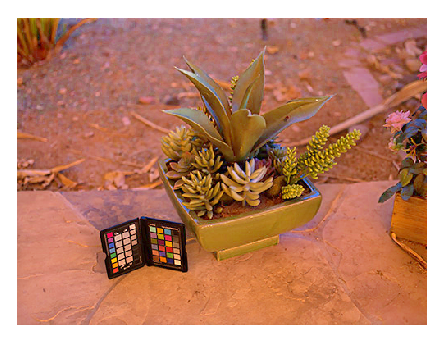
\includegraphics[width=35mm, height = 25mm]{images/experiment/parameter/reflectance/0.001-0.001.eps}
	\end{minipage}
	\begin{minipage}[b]{0.24\hsize}
		\centering
		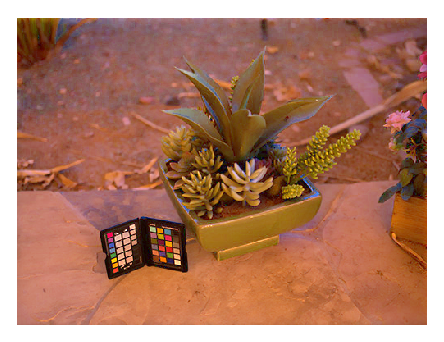
\includegraphics[width=35mm, height = 25mm]{images/experiment/parameter/reflectance/0.001-0.01.eps}
	\end{minipage}
	\begin{minipage}[b]{0.24\hsize}
		\centering
		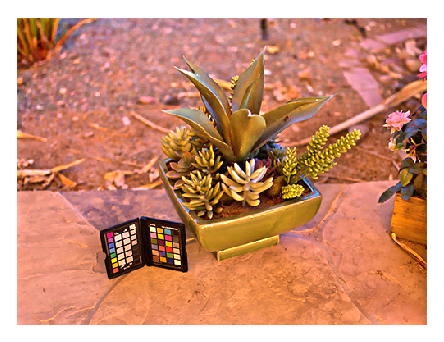
\includegraphics[width=35mm, height = 25mm]{images/experiment/parameter/reflectance/0.01-0.001.eps}
	\end{minipage}
	\begin{minipage}[b]{0.24\hsize}
		\centering
		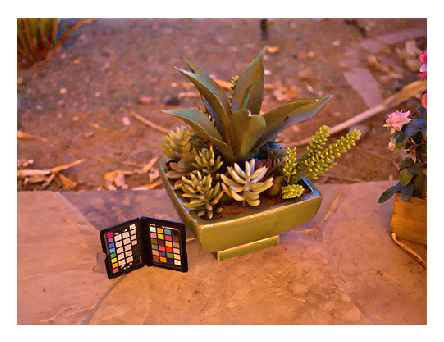
\includegraphics[width=35mm, height = 25mm]{images/experiment/parameter/reflectance/0.01-0.01.eps}
	\end{minipage}\\
	\vspace{3mm}
	\begin{minipage}[b]{0.24\hsize}
			\centering
			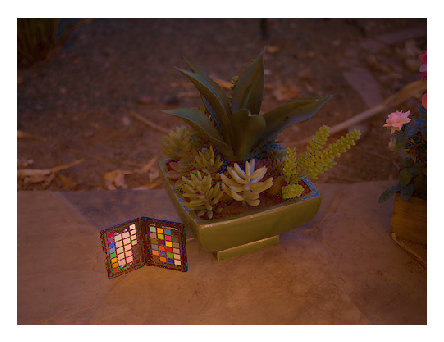
\includegraphics[width=35mm, height =25mm]{images/experiment/parameter/illumination/0.001-0.001.eps}
	\end{minipage}
	\begin{minipage}[b]{0.24\hsize}
			\centering
			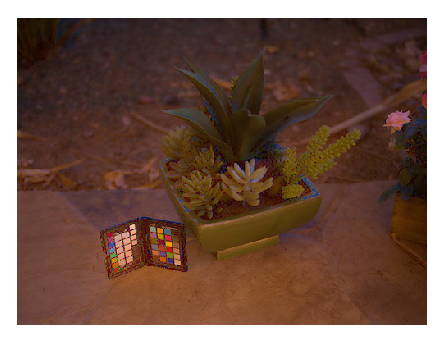
\includegraphics[width=35mm, height = 25mm]{images/experiment/parameter/illumination/0.001-0.01.eps}
	\end{minipage}
	\begin{minipage}[b]{0.24\hsize}
			\centering
			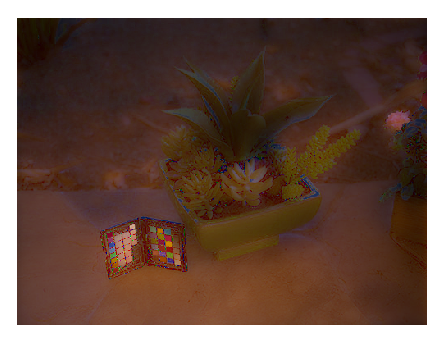
\includegraphics[width=35mm, height = 25mm]{images/experiment/parameter/illumination/0.01-0.001.eps}
	\end{minipage}
	\begin{minipage}[b]{0.24\hsize}
			\centering
			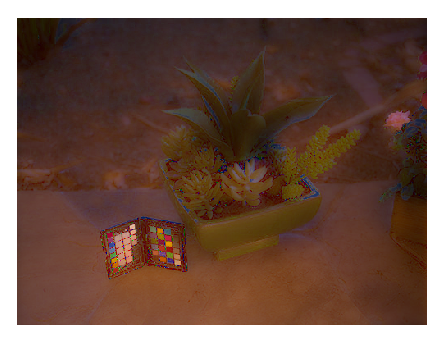
\includegraphics[width=35mm, height = 25mm]{images/experiment/parameter/illumination/0.01-0.01.eps}
	\end{minipage}\\
	\vspace{3mm}
	\begin{minipage}[b]{0.24\hsize}
			\centering
			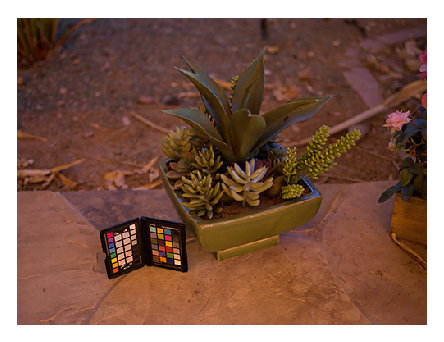
\includegraphics[width=35mm, height = 25mm]{images/experiment/parameter/output/0.001-0.001.eps}
			\subcaption{$(0.001, 0.001)$} \label{fig:parameter/qualitative/0001-0001}
	\end{minipage}
	\begin{minipage}[b]{0.24\hsize}
			\centering
			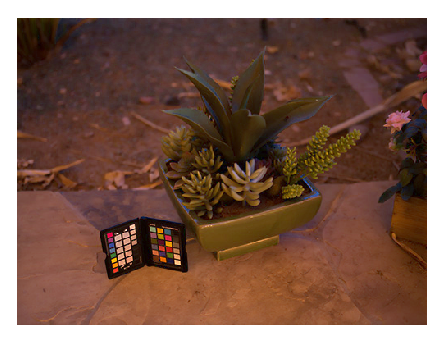
\includegraphics[width=35mm, height = 25mm]{images/experiment/parameter/output/0.001-0.01.eps}
			\subcaption{$(0.001, 0.01)$} \label{fig:parameter/qualitative/0001-001}
	\end{minipage}
	\begin{minipage}[b]{0.24\hsize}
			\centering
			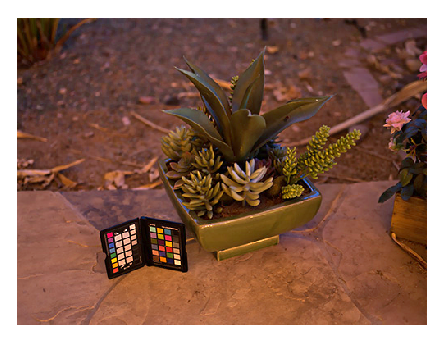
\includegraphics[width=35mm, height = 25mm]{images/experiment/parameter/output/0.01-0.001.eps}
			\subcaption{$(0.01, 0.001)$} \label{fig:parameter/qualitative/001-0001}
	\end{minipage}
	\begin{minipage}[b]{0.24\hsize}
			\centering
			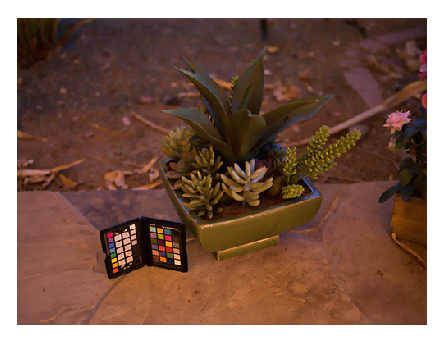
\includegraphics[width=35mm, height = 25mm]{images/experiment/parameter/output/0.01-0.01.eps}
			\subcaption{$(0.01, 0.01)$} \label{fig:parameter/qualitative/001-001}
	\end{minipage}\\
	\caption{Results for different results of $(\alpha, \beta)$ pairs. Top: reflectance. Middle: illumination. Bottom: enhanced images.}
	\label{fig:parameter/qualitative}
\end{figure}
%\subsection{Effect of the proposed method}
%In this section, the main purpose is to examine the effect of the proposed method. This experiment performs comparison with the proposed method and the methods, which do not adopt a $L_{P}$ norm as the constraint term on the illumination and do not add the adaptive texture map as the weight of the constraint term on the reflectance. The former is called "w/o $U$" method, and the latter is called "w/o $W$" method. Fig. \ref{fig:effect_prop} summarizes the impacts in the quantitative evaluations. It can be seen that these methods have lower average scores than the competitor such as SRIE and RRM, which has the second average score in each evaluation. This means that two weight matrices needs to keep the naturalness of the enhanced images. In addition, the proposed method results in the best average performance of all competing methods. This means that $U$ and $W$ influence each other in good was in the process of low-light image enhancement.
